\documentclass[12pt]{article}

\usepackage{graphicx}
\graphicspath{{Figures/}}
\usepackage{afterpage}
\usepackage{amsmath}
\usepackage{amsfonts}
\usepackage{amssymb}
\usepackage{amsbsy}
\usepackage{bm}
\usepackage{epsfig}
\usepackage{rotating}
\usepackage{setspace}
\usepackage{tabls}
\usepackage{hhline}
\usepackage{float}
\usepackage{subfigure}
\usepackage{subfigmat}
\usepackage{citesort}
\usepackage{cites}
\usepackage{overcite}                                                           
                                                 
% uncomment for submission of manuscript to NSE
%\usepackage[nolists, nomarkers]{endfloat}
%
% use to include postscript figures

%
%\usepackage[light,firsttwo]{draftcopy}
%\draftcopySetGrey{0.90}
                                                                                                            
%\usepackage{dbl}

\usepackage{diagbox}
% -----------------------------------------------------------------------------
% define newcommands
% -----------------------------------------------------------------------------

%\setlength{\floatsep}{4pt plus 1pt minus 1pt}
\setlength{\textfloatsep}{8pt plus 1pt minus 1pt}
%\setlength{\intextsep}{4pt plus 1pt minus 1pt}
\setlength{\abovedisplayskip}{4pt plus 1pt minus 1pt}
\setlength{\belowdisplayskip}{4pt plus 1pt minus 1pt}

\makeatletter
%\renewcommand{\@thesubfigure}{\thefigure\thesubfigure\space}
\makeatother
% =================================================================================================
% more new commands
% +++++++++++++++++++++++++++++++++++++++++++++++++++++++++++++++++++++++++++++++++++++++++++++++++
\setlength{\textwidth}{6.5in}
\setlength{\textheight}{8.5in}
\setlength{\oddsidemargin}{0in}
\setlength{\topmargin}{0pt}
\setlength{\headsep}{12pt}
%\addtolength{\oddsidemargin}{-0.5in}
%\addtolength{\textwidth}{1.0in}
%\addtolength{\textheight}{1.0in}
\renewcommand{\thefootnote}{\fnsymbol{footnote}}
%
% -----------------------------------------------------------------------------
% define newcommands
% -----------------------------------------------------------------------------

%\setlength{\floatsep}{4pt plus 1pt minus 1pt}
\setlength{\textfloatsep}{8pt plus 1pt minus 1pt}
%\setlength{\intextsep}{4pt plus 1pt minus 1pt}
\setlength{\abovedisplayskip}{4pt plus 1pt minus 1pt}
\setlength{\belowdisplayskip}{4pt plus 1pt minus 1pt}

% =================================================================================================
% more new commands
% +++++++++++++++++++++++++++++++++++++++++++++++++++++++++++++++++++++++++++++++++++++++++++++++++

% Ways of grouping things
%
\newcommand{\bracket}[1]{\left[ #1 \right]}
\newcommand{\bracet}[1]{\left\{ #1 \right\}}
\newcommand{\fn}[1]{\left( #1 \right)}
\newcommand{\ave}[1]{\left\langle #1 \right\rangle}
%
% Derivative forms
%
\newcommand{\dx}[1]{\,d#1}
\newcommand{\dxdy}[2]{\frac{\partial #1}{\partial #2}}
\newcommand{\dxdt}[1]{\frac{\partial #1}{\partial t}}
\newcommand{\dxdz}[1]{\frac{\partial #1}{\partial z}}
\newcommand{\dfdt}[1]{\frac{\partial}{\partial t} \fn{#1}}
\newcommand{\dfdz}[1]{\frac{\partial}{\partial z} \fn{#1}}
\newcommand{\ddt}[1]{\frac{\partial}{\partial t} #1}
\newcommand{\ddz}[1]{\frac{\partial}{\partial z} #1}
\newcommand{\dd}[2]{\frac{\partial}{\partial #1} #2}
\newcommand{\ddx}[1]{\frac{\partial}{\partial x} #1}
\newcommand{\ddy}[1]{\frac{\partial}{\partial y} #1}
%
% Vector forms
%
%\renewcommand{\vec}[1]{\ensuremath{\stackrel{\rightarrow}{#1}}}
%\renewcommand{\div}{\ensuremath{\vec{\nabla} \cdot}}
%\newcommand{\grad}{\ensuremath{\vec{\nabla}}}
\renewcommand{\vec}[1]{\overrightarrow{#1}}
\renewcommand{\div}{\vec{\nabla}\! \cdot \!}
\newcommand{\grad}{\vec{\nabla}}
\newcommand{\oa}[1]{\fn{\frac{1}{3}\hat{\Omega}\!\cdot\!\overrightarrow{A_{#1}}}}

%
% Equation beginnings and endings
%
\newcommand{\bea}{\begin{eqnarray}}
\newcommand{\eea}{\end{eqnarray}}
\newcommand{\be}{\begin{equation}}
\newcommand{\ee}{\end{equation}}
\newcommand{\beas}{\begin{eqnarray*}}
\newcommand{\eeas}{\end{eqnarray*}}
\newcommand{\bdm}{\begin{displaymath}}
\newcommand{\edm}{\end{displaymath}}
%
% Equation punctuation
%
\newcommand{\pec}{\hspace{0.25in},}
\newcommand{\pep}{\hspace{0.25in}.}
\newcommand{\pev}{\hspace{0.25in}}
%
% Equation labels and references, figure references, table references
%
\newcommand{\LEQ}[1]{\label{eq:#1}}
\newcommand{\EQ}[1]{Eq.~(\ref{eq:#1})}
\newcommand{\EQS}[1]{Eqs.~(\ref{eq:#1})}
\newcommand{\REQ}[1]{\ref{eq:#1}}
\newcommand{\LFI}[1]{\label{fi:#1}}
\newcommand{\FI}[1]{Fig.~\ref{fi:#1}}
\newcommand{\RFI}[1]{\ref{fi:#1}}
\newcommand{\LTA}[1]{\label{ta:#1}}
\newcommand{\TA}[1]{Table~\ref{ta:#1}}
\newcommand{\RTA}[1]{\ref{ta:#1}}

%
% List beginnings and endings
%
\newcommand{\bl}{\bss\begin{itemize}}
\newcommand{\el}{\vspace{-.5\baselineskip}\end{itemize}\ess}
\newcommand{\ben}{\bss\begin{enumerate}}
\newcommand{\een}{\vspace{-.5\baselineskip}\end{enumerate}\ess}
%
% Figure and table beginnings and endings
%
\newcommand{\bfg}{\begin{figure}}
\newcommand{\efg}{\end{figure}}
\newcommand{\bt}{\begin{table}}
\newcommand{\et}{\end{table}}
%
% Tabular and center beginnings and endings
%
\newcommand{\bc}{\begin{center}}
\newcommand{\ec}{\end{center}}
\newcommand{\btb}{\begin{center}\begin{tabular}}
\newcommand{\etb}{\end{tabular}\end{center}}
%
% Single space command
%
%\newcommand{\bss}{\begin{singlespace}}
%\newcommand{\ess}{\end{singlespace}}
\newcommand{\bss}{\singlespacing}
\newcommand{\ess}{\doublespacing}
%
%---New environment "arbspace". (modeled after singlespace environment
%                                in Doublespace.sty)
%   The baselinestretch only takes effect at a size change, so do one.
%
\def\arbspace#1{\def\baselinestretch{#1}\@normalsize}
\def\endarbspace{}
\newcommand{\bas}{\begin{arbspace}}
\newcommand{\eas}{\end{arbspace}}
%
% An explanation for a function
%
\newcommand{\explain}[1]{\mbox{\hspace{2em} #1}}
%
% Quick commands for symbols
%
\newcommand{\half}{\frac{1}{2}}
\newcommand{\third}{\frac{1}{3}}
\newcommand{\twothird}{\frac{2}{3}}
\newcommand{\mdot}{\dot{m}}
\newcommand{\ten}[1]{\times 10^{#1}\,}
\newcommand{\cL}{{\cal L}}
\newcommand{\cD}{{\cal D}}
\newcommand{\cF}{{\cal F}}
\newcommand{\cE}{{\cal E}}
\newcommand{\cS}{{\cal S}}
\newcommand{\mA}{\mathbf{A}}
\newcommand{\mX}{\mathbf{X}}
\newcommand{\mU}{\mathbf{U}}
\newcommand{\mW}{\mathbf{W}}
\newcommand{\mSigma}{\mathbf{\Sigma}}
\newcommand{\mS}{\mathbf{S}}
\newcommand{\mB}{\mathbf{B}}
\newcommand{\mC}{\mathbf{C}}
\newcommand{\mD}{\mathbf{D}}
\renewcommand{\Re}{\mbox{Re}}
\newcommand{\Ma}{\mbox{Ma}}
%
% Inclusion of Graphics Data
%
%\input{psfig}
%\psfiginit
%
% More Quick Commands
%
\newcommand{\bi}{\begin{itemize}}
\newcommand{\ei}{\end{itemize}}
\newcommand{\dxi}{\Delta x_i}
\newcommand{\dyj}{\Delta y_j}
\newcommand{\ts}[1]{\textstyle #1}
% =================================================================================================
\date{}

\begin{document}

%\bibliographystyle{nse}
%\bibnum{p}

\thispagestyle{empty}

\bss
\bc
{\Large \bf Dynamic Mode Decomposition for Subcritical Metal Systems}\\
\vspace{0.3in}
{\large Zachary Hardy and Jim E. Morel\\
Texas A\&M University\\
Department of Nuclear Engineering\\
TAMU 3133\\
College Station, TX 77843-3133\\
$ $\\
Cory Ahrens\\
Los Alamos National Laboratory\\
Los Alamos, NM  87545\\
$ $\\
}
\emph{zach.hardy@tamu.edu, morel@tamu.edu, cdahrens@lanl.gov}

\vspace{1.5in}

Send proofs and page charges to:\\
\vspace{0.1in}
Dr. Jim Morel\\
Texas A\&M University\\
Department of Nuclear Engineering\\
TAMU 3133\\
College Station, TX 77843-3133\\
\vspace{0.25in}
25 Pages -- 1 Table -- 4 Figures \\
\ec
\ess

% =================================================================================================

\newpage

\begin{abstract}
In this paper we explore the use of Dynamic Mode Decomposition (DMD) for
	modeling the kinetics of subcritical metal systems pulsed with fast neutrons.
Our ultimate purpose is to obtain a fast and accurate reduced-order model for 
	such systems that can be used to develop an emulator.  
An alternative to DMD is $\alpha$-eigenfunction expansions, but we show that
	DMD is vastly superior in several ways for the systems of interest to us. 
\end{abstract}

\section{Introduction}
Modeling of subcritical metal systems subjected to short bursts of fast 
	neutrons is challenging. 
While such modeling can certainly be done with a time-dependent transport code, 
	we want to develop a reduced-order model that can provide physical insight 
	into such systems and form the basis of an emulator in order to solve inverse 
	problems quickly and compute sensitivities economically. 
One method of developing a reduced-order model is a truncated
	$\alpha$-eigenfunction expansion. 
To the author's knowledge, no proof of the incompleteness of the alpha 
	eigenfunctions exists. 
It seems, however, that because of the singular nature of the uncollided and    
	first collided flux (cite Larsen and Bondarenko), the $\alpha$-eigenfunctions likely do not form a 
	complete basis. 
However, Jorgens proved, under rather general assumptions, that the 
	$\alpha$-eigenfunctions form an ``asymptotically complete'' basis in the 
	following sense: for times $t>3\tau$, where $\tau$ is a representative time 
	for neutrons to stream across the spatial domain, $\psi\left(t\right) \sim 
	\sum_{n=0}^{N-1} A_n \psi_n e^{\alpha_n t}$, where the remainder term is 
	proportional to $e^{\alpha_N t}$ and the amplitudes $A_n$ depend on the 
	initial condition. 
From this representation and the fact that the eigenvalues are ordered as 
	$...Re\left(\alpha_3\right)\le Re\left(\alpha_2\right)\le  Re\left(\alpha_1\right) < \alpha_0$, one sees that 
	$|\alpha_0 - \alpha_1|^{-1}$ sets a time scale for the higher-order modes to 
	decay relative to the fundamental mode. 
The relationship of this time scale compared with the time over which the 
	experiment takes place can be significantly different for subcritical 
	compared to supercritical systems.  

Indeed, for a supercritical system, where $\alpha_0 > 0$ and the real part of 
	$\alpha_n$, $n=1,2,3,...$ is negative, the transport solution is quickly 
	dominated by the fundamental mode $\alpha$-eigenfunction.
However, the situation can be different for a subcritical system. 
If the flux (experimental signal) decays much faster than $|\alpha_0 - 
	\alpha_1|^{-1}$, then the fundamental mode might not contribution 
	significanlty to the signal before it is negligibly small. 
The contribution of the fundamental mode depends upon the extent to which it is 
	present in the expansion for the initial condition. 
In a subcritical system the fundamental mode will be dominated by the slowest 
	neutrons, which will be thermal neutrons. 
In a metal system subjected to a burst of fast neutrons, there will be almost 
	no thermal neutrons created before the response of the system has effectively 
	died away.  
Thus it seems likely that an $\alpha$-eigenfunction expansion will be 
	particularly inefficient for such systems, because a high degree of 
	cancellation between the eigenfunctions will be required to achieve a 
	negligible thermal neutron component in the initial condition.  

Dynamic Mode Decomposition (DMD) is a reduced order technique for modeling
	dynamical systems.
It has been applied in many areas and is perhaps best known for its use in the 
	fluid-flow community 
	\cite{dmd2016}$^,$\cite{schmid2010}$^,$\cite{jovanovic2012low} .
The purpose of this paper is to perform a preliminary investigation of DMD as 
	an alternative to $\alpha$-eigenfunction expansions for modeling pulsed 
	neutron experiments \cite{abdo2018}$^,$\cite{rm} .
For this initial study, we use a very approximate but relevant high-dimensional 
	model consisting of a time-dependent 1-D spherical geometry three-group 
	diffusion approximation. 
We have an analytic eigenfunction solution for these equations, as well as a 
	computer code for solving these equations with second-order accuracy in both 
	time and space.  
We later describe DMD in detail, but at this point it suffices to say that 
	given a time series of vector ``snapshots'' from a simulation or experiment, 
	DMD produces a time-dependent solution for those snapshots that is 
	constructed from a sum of snapshot modes, each with an exponential decay rate.
For instance, the snapshots could be space-dependent, three-group diffusion 
	scalar fluxes from a time-dependent calculation.  
They could also be an analogous time series of any quantity of interest 
	computed from the diffusion solution, such as space-dependent reaction rates.
The form of the DMD solution is identical to that of an alpha-eigenfunction  
	solution.  
However, the DMD modes can only contain what the snapshots contain, so if the 
	snapshots lack a thermal neutron component, so will the DMD modes.
This suggests that fewer DMD modes should be required for our problems than
	$\alpha$-eigenfunctions.

Indeed we present results demonstrating that the DMD method is accurate and 
	more efficient than $\alpha$-eigenfunction expansions for our problems.  
The remainder of this paper is organized as follows.  
First we describe the particular variant of the DMD method that we use.  
Then we describe the three-group diffusion model, followed by a description of 
	our space-time discretization for the diffusion model.  
Finally, numerical results are given, followed by conclusions and 
	recommendations for future work.

\section{The DMD Method}
There are many variations of the DMD method.  
Here we describe the variant that we use to model subcritical fissioning 
	systems \cite{dmd2016}$^,$\cite{schmid2010} .
One begins with a time series of vector snapshots, $\{\vec{v}_j\}_{j=1}^{N}$, 
	uniformly sampled in time, that are associated with the dynamical system. 
We assume that at least the first $N-1$ snapshots are linearly-independent. 
A process for ensuring this is later discussed.  
Each vector has $M$ real components with $M \gg N$. 
For example, each snapshot could represent a discrete angular flux solution in 
	a time-dependent transport calculation, or it could represent some 
	space-dependent quantity of interest associated with that solution.  
Note that the snapshots can be obtained either computationally or 
	experimentally. 
For our application, we generate them computationally. 
It is further assumed that there exists a temporal matrix $\mathbf{A}$, that 
	maps each snapshot to its successor:

\be
	\vec{v}_{i+1} = \mA \vec{v}_{i} \pec \quad i=1,N-1.
	\LEQ{2.1}
\ee
Let us consider the subspace of $M$-vectors, which we denote by $\cS$, spanned 
	by the first $N-1$ snapshots.  
If $\vec{v}_N$ were replaced by a least-squares fit from $\cS$, then $\mA$ 
	would be uniquely defined as a mapping from $\cS$ to $\cS$, and be 
	represented by the following matrix with respect to the snapshot basis:

\be
	\mA_s = \bracket{
	\begin{array}{ccccccc}
		0 & 0 & ....& 0 & c_1 \\
		1 & 0 & ....& 0 & c_2 \\
		0 & 1 & ....& 0 & c_3 \\
		. & . & ....& . & . \\
		. & . & ....& . & . \\
		. & . & ....& . & . \\
		0 & 0 & ....& 0 & . \\
		0 & 0 & ....& 1 & c_{N-1}
	\end{array}
	} \pec
	\LEQ{2.2}
\ee
where the least-squares fit to $\vec{v}_N$ from $\cS$ is represented by

\be
	\widehat{v}_N = \sum_{j=1}^{N-1} c_j \vec{v}_j \pep
	\LEQ{2.3}
\ee
For example, in the snapshot basis,

\be
	\vec{v}_1 = (1,0,0,0,...0)^T \pec
	\LEQ{2.4}
\ee
and 
\be
	\mA \vec{v}_1 = \vec{v}_2 = (0,1,0,0,...0)^T \pec
	\LEQ{2.5}
\ee
Note that if $c_1$ is non-zero, $\mA$ will be invertible on $\cS$, and thus 		
	will have $N-1$ non-zero eigenvalues. 
We will define $\mA$ in this manner with respect to $\cS$, assume that it is 
	invertible on $\cS$, and further define all of its remaining eigenvalues to 
	be zero.  
Let $\{\lambda_i\}_{i=1}^{N-1}$ denote the non-zero eigenvectors of $\mA$, and 
	let $\{\vec{z}_i\}_{i=1}^{N-1}$ denote the corresponding eigenvectors. 
Then the dynamic solution is given by 

\be
	\vec{v}(t) = \sum_{i=1}^{N-1} a_i \vec{z}_i \exp{(\omega_i t)} \pec
	\LEQ{2.5a}
\ee
where
 
\be
	\omega_i = \frac{\ln{(\lambda_i)}}{\Delta t} \pec
	\LEQ{2.5b}
\ee
where $\Delta t$ is the time between snapshots and the expansion coefficients, 
	$\{a_i\}_{i=1}^{N-1}$ are determined by the initial condition:
 
\be
	\vec{v}(0) = \vec{v}_1 = \sum_{i=1}^{N-1} a_i \vec{z}_i \pep
	\LEQ{2.5c}
\ee
The dynamic solution exactly reproduces each of the snapshots at its time of 
	sampling with the exception of the last snapshot, which is approximated with 
	its least-squares fit. 
This follows from the fact that at the end of the first sampling period, $\mA$ 
	is effectively applied to $\vec{v}_1$, and reapplied at the end of each 
	sampling period thereafter.  
For instance, 

\bea
	\vec{v}(\Delta t) &=& \sum_{i=1}^{N-1} a_i \vec{z}_i \exp{(\omega_i \Delta t)} \pec \nonumber \\
	&=& \sum_{i=1}^{N-1} a_i \vec{z}_i \lambda_i \pec \nonumber \\ 
	&=& \mA \vec{v}_1 \pec \nonumber \\ 
	&=& \vec{v}_2 \pep
	\LEQ{2.5d}
\eea 
Note that any eigenfunction with a zero-eigenvalue will have no dynamic content 
	because it will instantly attenuate to zero.  
Thus if $\widehat{v}_N$ has a zero value for $c_1$ in \EQ{2.3}, $\mA$ will have 
	only $N-2$ non-zero eigenvalues, and one can simply ignore the eigenfunction 
	associated with the extra zero eigenvalue.  
We henceforth continue to assume that $\mA$ has $N-1$ non-zero eigenvalues for 	
	simplicity, but without loss of generality.

We now describe a process that enables us to compute the non-zero eigenvalues 
	and the eigenvectors of $\mA$.  
Furthermore, we need not explicitly compute $\widehat{v}_N$.
First we express \EQ{2.1} as follows, neglecting the substitution of 
	$\widehat{v}_N$ for $\vec{v}_N$ for reasons later explained. 

\be
	\mX_2^{N} = \mA \mX_{1}^{N-1} \pec
	\LEQ{2.6}
\ee
where $\mX_2^{N}$ is the $M \times N-1$ matrix whose colunms are the vectors 		
	$\vec{v}_2$ through $\vec{v}_{N}$, and $\mX_{1}^{N-1}$ is the $M\times N-1$ 
	matrix whose colunms are the vectors $\vec{v}_1$ through $\vec{v}_{N-1}$. 

We next perform a singular value decomposition (SVD) of $\mX_{1}^{N-1}$:

\be
	\mX_{1}^{N-1} = \mU \mSigma \mW^T \pec
	\LEQ{2.7}
\ee
where $\mU$ is a $M \times M$ orthogonal matrix, $\mSigma$ is a $M\times N-1$ 
	matrix with $N-1$ non-zero singular values on the diagonal and zeros 
	everywhere else, and $\mW^T$ is a $N-1 \times N-1$ orthogonal matrix.  
Substituting from \EQ{2.6} into \EQ{2.7}, we obtain, 

\be
	\mX_2^{N} = \mA \mU \mSigma \mW^T \pec
	\LEQ{2.8}
\ee
Next we multiply \EQ{2.8} on the left by $\mU^{T}$ and on the right by 
	$\mW\mSigma^{-1}$ to obtain 

\be
	\mS = \mU^{T}\mX_2^{N}\mW\mSigma^{-1} = \mU^{T}\mA\mU \pec
	\LEQ{2.10}
\ee
where $\mSigma^{-1}$ is the pseudo inverse of $\mSigma$.
The pseudo-inverse is obtained from $\mSigma$ simply by first inverting its 
	non-zero elements and then transposing it. 
Note that the right side of \EQ{2.10} is a $M \times M$ matrix that represents 
	a similarity transformation of $\mA$, and thus $\mS$ has the same eigenvalues 
	as $\mA$.  
Furthermore, in accordance with the similarity transformation, if $\vec{y}$ is 
	an eigenvector of $\mS$, then $\vec{z} = \mU \vec{y}$ is an eigenvector of 
	$\mA$.  

The structure of $\mS$ is important because it enables us to avoid computing 
	the entire $M \times M$ matrix together with its eigenvalues and eigenvectors.
More specifically, all the columns of $\mS$ beyond column $N-1$ are zero, and 
	we represent the remainder of the matrix as an $N-1 \times N-1$ matrix, 
	$\mS_{T}$, in the upper top left corner and a $M-N+1 \times N-1$ matrix, 
	$\mS_B$, in the bottom left corner:
 
\be
	\mS = \bracket{
	\begin{array}{cc}
		\mS_T  & 0 \\
		\mS_B & 0  
	\end{array}
	} \pec
	\LEQ{2.11}
\ee
It can be shown that the eigenvalues of $\mS_T$ are the non-zero eigenvalues of 
	$\mS$, and hence, the non-zero eigenvalues of $\mA$.  
Furthermore, there is a very simple way to compute the corresponding 
	eigenvectors of $\mS$ from the eigenvectors of $\mS_T$. 
However, it is unnecessary to compute any eigenvectors other than those of 
	$\mS_T$.  
To explain why this is so, we first note that the there is no difference 
	between the eigenvectors of $\mS_T$ and the vectors formed by the first $N-1$ 
	components of the corresponding eigenvectors of $\mS$.  
Thus if one computes the eigenvalues and eigenvectors of $\mS_T$, one has the 
	non-zero eigenvalues of $\mA$ and $\mS$, and the corresponding eigenvectors 
	of $\mS$ truncated to a length of $N-1$.

The first step in the calculation of the non-zero eigenvalues and corresponding 
	eigenvectors of $\mA$ is to directly compute $\mS_T$ as follows:

\be
	\mS_T = \mU_{N-1}^{T} \mX_{2}^{N}\mW\mSigma^{-1}_{N-1} \pec
	\LEQ{2.12}
\ee
where $\mU_{N-1}$ is the $M \times N-1$ matrix composed of the first $N-1$ 
	columns of $\mU$, and $\mSigma_{N-1}$ is the $N-1 \times N-1$ matrix formed 
	by the first $N-1$ rows of $\mSigma$.  

At this point we have sufficient information to explain why one need not 
	substitute $\widehat{v}_N$ for $\vec{v}_N$ in $\mX_2^{N}$.  
To this end we express the equations for the expansion coefficients of the 
	least-squares fit to $\vec{v}_N$ as follows:

\be
	\mU^T_{N-1}\fn{\widehat{v}_N - \vec{v}_N} = \vec{0} \pec
	\LEQ{2.9}
\ee
where $\mU_{N-1}$ is the $M \times N-1$ matrix consisting of the first $N-1$ 
	columns of $\mU$. 
Note that by virtue of the SVD of $\mX_{1}^{N-1}$, these column vectors 
	represent an orthonormal basis for the first $N-1$ snapshots.  
Thus $\widehat{v}_N$ does indeed represent a least-squares fit to $\vec{v}_N$
	from $\cS$.  
From \EQ{2.9} it follows that the first $N-1$ components of $\mU^T \vec{v}_N$ 
	are identical to those of $\mU^T \widehat{v}_N$. 
Thus it can be seen from \EQ{2.12} that $\mS_T$ is invariant to the 
	substitution of $\widehat{v}_N$ for $\vec{v}_N$ in $X_{2}^{N}$.

Finally, we compute the non-zero eigenvectors of $\mA$ simply by multiplying 
	the eigenvectors of $\mS_T$ by $U_{N-1}$. 

\be
	\vec{z}_i = \mU_{N-1} \vec{x}_i \pec \quad i=1,N-1,
	\LEQ{2.13}
\ee
where $\vec{z}_i$ and $\vec{x}_i$ are the $i$'th eigenvectors of $\mA$ and 
	$\mS_T$, respectively.  
This is clearly much more economical than computing the eigenvectors of $\mS$ 
	and multiplying them by $\mU$.  
This simplification is justified by the fact that since the first $N-1$ columns 
	of $\mU$ form an orthonormal basis for $\cS$, the non-zero eigenvectors of 
	$\mA$ must lie in this space.  
Thus columns of $\mU$ beyond $N-1$, or equivalently, elements of the  
	eigenvectors of $\mS$ below the $N-1$ position do not contribute to the 
	non-zero eigenvectors of $\mA$. 

As previously discussed, the SVD of $\mX_{1}^{N-1}$ can be used to determine if 
	the first $N-1$ snapshots are sufficiently linearly independent by inspection 
	of the singular values.  
Below some tolerance, one can consider the singular values to be zero, and 
	discard the corresponding information in the various component matrices. 
More specifically, if we assume that only the first $K$ singular values are 
	considered non-zero, then in \EQ{2.12} only the first $K$ columns of 
	$\mU_{N-1}$ and $\mX_{2}^{N}$ are retained, and only the first $K$ columns 
	and first $K$ rows of $\mSigma_{N-1}$ and $\mW^T$ are retained.  
We currently set any singular value that is less than $10^{-8}$ times the 
	largest singular value to zero. 
It is not generally clear as to what tolerance is the most efficient.  
We determine this on a case-by-case basis.

\section{The Three-Group Diffusion Model}
The primary goal of this work is to explore the ability of DMD to effectively 
	filter out irrelevant portions of phase space to produce a reduced order 
	model.  
Because thermal neutrons have effectively no contribution to the results of a 
	computational model or experiment within the application space of interest, 
	we choose the model to reflect these characteristics. 
For the purposes of this  work, only diffusion in a bare, homogeneous 
	fissioning sphere with an atom density of $N = 0.05 \text{ atoms/cc}$ is 
	considered. 

For simplicity, and to give a clear DMD performance metric, three energy groups 
	- fast, epithermal, and thermal - are used.  
The nuclear data is tabulated in \TA{xs_data}, where $\chi$ is the fission 
	spectrum, $\nu\sigma_f$ is the fission neutron production cross section, 
	$\sigma_R$ is the removal cross section, including absorption and 
	outscattering, $\sigma_t$ is the total cross section, and $v$ is the velocity.
As is apparent from the table, fission neutrons are only born into the fast 
	group indicating that the only production of epithermal and thermal neutrons 
	comes from downscattering. 
The scattering matrix is shown in \TA{scat}.  
There is only scattering from the fast to epithermal group and no upscattering 
	whatsoever.  

With this model it is assured that thermal neutrons only appear in the problem 
	if they exist in the initial condition.  
This makes the analysis of the performance of the DMD quite simple; in a 
	problem where thermal neutrons are, in fact, irrelevant to the solution, the 
	DMD solution should not have a thermal component. 

\bt[h] \centering 
	\caption{Nuclear data for the three-group model.} 
	\btb{|c|c|c|c|}
		\hline
		\diagbox{Reaction}{Group} & Fast  & Epithermal  & Thermal  \\  \hline
		$\chi$  & 1 & 0 & 0 \\ 	\hline
		$\nu\sigma_f \ [b]$ & 5.4 & 60.8 & 28.0 \\  \hline
		$\sigma_R \ [b]$  & 3.31 & 36.2 & 13.6 \\  \hline
		$\sigma_t \ [b]$ & 7.71 & 50.0 & 25.6\\ \hline
		$v \ [cm/\mu s]$ & 2000 & 100 & 2.2 \\  \hline
	\etb  \LTA{xs_data}
\et

\bt[h] \centering 
	\caption{Scattering matrix given in barns.} 
	\btb{|c|c|c|c|}
		\hline
		\diagbox{From}{To}& Fast  & Epithermal  & Thermal  \\  \hline
		Fast  & 0 & 1.46 & 0 \\  \hline
		Epithermal & 0 & 0 & 0 \\  \hline
		Thermal  & 0 & 0 & 0 \\  \hline
	\etb \LTA{scat}
\et

This system is governed by the time-dependent multi-group neutron diffusion 
	equations. 
The center of the spherical system is reflective and a zero-flux condition is 
	imposed at the physical boundary. 
The initial condition will be parabolic in space for both the fast and 
	epithermal groups and zero for the thermal group. 
This is given in \EQ{mg_diff},

\be
	\begin{cases}
		\dxdy{\phi_g}{t} - \nabla \cdot D_g \nabla \phi_g + \Sigma_{R,g} \phi_g 
			= \chi_g \sum\limits_{g'=1}^{3} \nu\Sigma_{f,g'} \phi_{g'} + 
		 	\sum\limits_{g'=1, \ g' \neq g}^g \Sigma_s^{g' \rightarrow g} \phi_{g'} \\
		-D_g \dxdy{\phi_g}{r} \Big\rvert_{(0,t)} = 0, \pev \phi_g(R,t) = 0 \\
			\phi_1(r,0) = \phi_2(r,0) = \frac{R^2 - r^2}{R^2}, \pev \phi_3(r,0) = 0
	\end{cases} ,
	\LEQ{mg_diff}
\ee 
where $\Sigma$'s are macroscopic cross sections, given by $\Sigma = N\sigma$, 
	and $D_g$ is the diffusion coefficient, given by $1/3\Sigma_t$. 
This can be simplified based on the nuclear data to \EQ{simp_diff}.

\be
	\begin{cases}
		\dxdy{\phi_g}{t} - \nabla \cdot D_g \nabla \phi_g + \Sigma_{R,g} \phi_g 
			= \chi_1 \sum\limits_{g'=1}^{3} \nu\Sigma_{f,g'} \phi_{g'} + 
			\Sigma_s^{1 \rightarrow 2} \phi_{1} \\
		-D_g \dxdy{\phi_g}{r} \Big\rvert_{(0,t)} = 0, \pev \phi_g(R,t) = 0 \\
		\phi_1(r,0) = \phi_2(r,0) = \frac{R^2 - r^2}{R^2}, \pev \phi_3(r,0) = 0.
	\end{cases} 
	\LEQ{simp_diff}
\ee

This problem can be solved using an doubly-indexed $\alpha$-eigenfunction 
	expansion.  
The expansion takes the form shown in \EQ{exp},

\be
	\phi_g(r, t) = \sum_{n, m = 1}^{\infty, 3} A_{nm} \varphi_n(r) f_{nm, g} e^{\alpha_{nm} t},
\LEQ{exp} \ee
where $n$ gives the index of the spatial mode and $m$ gives the index of the 
	energy modes corresponding to each spatial mode.
$A_{nm}$ is the coeffient for the $n,m$'th space-energy mode, $\varphi_n(r)$ is 
	the $n$'th spatial mode, $f_{nm, g}$ is the $g$'th component of the $n,m$'th 
	space-energy mode, and $\alpha_{nm}$ is the time eigenvalue for the $n,m$'th 
	space-energy mode. 
The spatial modes are those of the Laplace equation for a spherical geometry 
	given by \EQ{eigfunc}, with the same boundary conditions as those in the 
	governing equation.

\be
	\varphi_n(r) = \frac{1}{r} \sin\fn{ \frac{n \pi r}{R} }
	\LEQ{eigfunc}
\ee

For simplicity, the buckling approximation is used in place of the Laplacian, 
	as shown in \EQ{buckle}.

\bea 
	\begin{aligned}
		- \nabla^2 \varphi_n(r) &= B_n^2 \varphi_n(r) \\
	 	B_n^2 &= \fn{ \frac{n \pi}{R} }^2
	\end{aligned} 
	\LEQ{buckle} 
\eea
Plugging in the eigenfunction expansion into the governing equation, 
	rearranging, and taking advantage of the orthogonality of the spatial 
	eigenfunctions, an eigenvalue problem is formed for each spatial mode, given 
	by \EQ{eigprob}.

\be
	\alpha_{nm} f_{nm, g} = v_g \fn{ - \fn{ D_g B_n^2 + \Sigma_{R,g} }f_{nm, g} 
		+ \chi_1 \sum_{g' = 1}^{3} \nu\Sigma_{f,g'} f_{nm, g'} 
		+ \Sigma_s^{1 \rightarrow 2} f_{nm, 1} } 
	\LEQ{eigprob}
\ee
It should be clear that this forms a 3 $\times$ 3 system which will yield 3 
	distinctive $\alpha$-eigenvalues with corresponding eigenvectors of length 3 
	for each spatial mode used in the expansion.

The coefficients for each space-energy mode is computed by a projection of the 
	the initial condition onto each respective space-energy mode. 
Because the eigenproblem described above is not symmetric, the adjoint (left) 
	eigenfunctions given by, $f_{nm}^* \varphi_n(r)$, must be used. 
The spatial eigenfunctions do not have the adjoint designation because they are 
	self-adjoint. 
The coefficients are computed according to \EQ{coeff},

\be
	A_{nm} = \frac{\ave{ f_{nm}^* \varphi_n(r), \ \phi(r, 0)}}{\ave{f_{nm}^* 	
			\varphi_n(r), \ f_{nm} \varphi_n(r)}},
	\LEQ{coeff} 
\ee
where $\ave{\cdot}$ designates the inner product, an integration and sum, over 
	space and energy, respectively. 
To generate the full analytic solution modes are generated and added to the 
	solution until the $L^2$-fit to the initial condition changes by less than a 
	specified tolerance. 
This expansion is then propegated forward in time with the
	$\alpha$-eigenfunctions to some specified time.

\section{Discretization of the Diffusion Equations}
In practice,  $\alpha$-eigenvalue calculations for this application are quite 
	computationally expensive, and  further, in most cases, analytic solutions is 
	not available. 
For this reason, it is desireable to develop a numerical method so that the 
	accuracy of DMD can be characterized in a realistic way and compared against 
	a known solution. 
This section outlines the development of a second-order accurate method using 
	cell-centered finite volume discretization in space and trapezoidal 
	second-order backwards difference (TBDF-2) discretization in time.

In the spatial discretization, the domain is broken into $N$ cells, with cell 
	width $h$, where the cell centers carry integer indiced and the edges 
	half-integer indices. 
Consider \EQ{cell_eqn}, the conservation equation for the i$^{\text{th}}$ cell,

\be
	 \frac{1}{v_g} \dxdt{\phi_{i,g}} - \nabla D_{g} \nabla \phi_{i,g} + 	
	 	\Sigma_{R,g} \phi_{i,g}  =  S_{i,g},
	\LEQ{cell_eqn} 
\ee
where $S_{i,g}$ contains the production terms for group $g$ neutrons in cell 		
	$i$.
The reader should note that source term is simply the fission and scattering 
	source.

\be
	\frac{V_i}{v_g} \dxdt{\phi_{i,g}} - A_{i+\half} J_{i+\half,g} + A_{i-\half} 
		J_{i-\half,g} + V_i \Sigma_{R,g} \phi_{i,g} = V_i S_{i,g}
\ee
where $V_i $ is the volume of cell $i$, $ A_{i+1/2} $ is the surface area of 
	the outer edge of cell $i$, and $ J_{i+1/2} = D_g \nabla \phi_{g,i} $ is the 
	current at outer edge of cell $i$. 
Central difference is now applied to the current terms with respect to adjacent 
	cell-centers to obtain the second-order accurate scheme, as shown in 
	\EQ{space_discretized}.

\be
	\frac{V_i}{v_g} \dxdt{\phi_{i,g}} - A_{i+\half} \frac{\phi_{i+1,g} - 
		\phi_{i,g}}{h} + A_{i-\half} \frac{\phi_{i,g} - \phi_{i-1,g}}{h} + 
		V_i \Sigma_{R,g} \phi_{i,g} = V_i S_{i,g},
 	\LEQ{space_discretized} 
\ee

The TBDF-2 temporal discretization is advantageous because it is second-order 
	accurate and strongly damps fast time-scale components of the solution, 
	unlike methods such as Crank-Nicholson, which can be highly oscillatory for 
	stiff systems. 
This method first takes half of a time-step using Crank-Nicholson, and is shown 
	for an arbitrary linear system in \EQ{halfCN}. 

\be
	\frac{2 \fn{ f^{n+\half} - f^n }}{\Delta t} =  \half A \fn{f^{n+\half} + f^n}.
	\LEQ{halfCN} 
\ee
The result of solving for $f^{n+\half}$ is then plugged into second-order 
	backwards difference to obtain the solution at the end of the time step, 
	shown in \EQ{halfBDF}.

\be
	\frac{3 \fn{ f^{n+1} - f^{n+\half} }}{\Delta t} - \frac{f^{n+\half} - 
		f^n}{\Delta t} = A f^{n+1}.
	\LEQ{halfBDF} 
\ee 
Implementing this is relatively straightforward. 
The time derivative term containing the scalar flux at ther next half-time step 
	gets added into the operator and the terms containing the scalar flux from 
	previous time-steps become a source term.

Overall, this method is second order accurate and was verified against the 
	analytic solution. 
\FI{2ord} shows the error as a function of number of spatiotemporal grid 
	halvings, where a slope of 2 is observed.

\bfg[h] \centering
	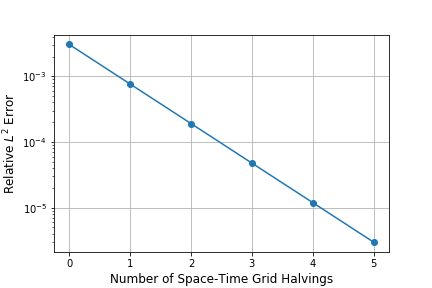
\includegraphics[scale=0.5]{method_convergence.png}
	\caption{Convergence of the numerical solution to the analytical}
	\LFI{2ord}
\efg

\section{Numerical Results}
In this section numerical results are presented which characterize the 
	efficiency and accuracy of DMD for this application using both the scalar 
	group flux and fission rate.
The DMD solution presented in this section is derived from data produced by the 
	numerical model discussed above for a 5 cm sphere over a 10 ns simulation 
	time discretized into 500 spatial cells and 30 time-steps.
Seperate sections will describe the application of DMD on both the scalar 
	group flux and the fission rate.
Each section will present the singular value spectrum for the simulation data,
	show the convergence of the DMD solution to the simulation data in the 
	Frobenius norm, show a few snapshots of the DMD solution overlayed on the 
	exact solution, and give results for the interpolative and extrapolative 
	abilities of DMD between snapshots and beyond the data collection period, 
	respectively.
In addition, the performance of DMD on the scalar group flux will and the 
	physical insights gained will be compared with that of an 
	$\alpha$-eigenfunction computation.

\subsection{DMD with the Scalar Group Flux}
In order for DMD to be a viable reduced order model, a low-rank structure must 
	exist within the data.
Because singular values are related to the eigenvalues matrix it decomposes, 
	the singular values of the rectangular matrix $\bm{X}^{N-1}_1$ contains 
	information about the dominant time-eigenvalues during the duration of the 
	simulation.
The singular value spectrum of  $\bm{X}^{N-1}_1$ is presented below in 
	\FI{sv-spec}, and shows that this condition is, in fact, met.

\bfg[h] \centering
	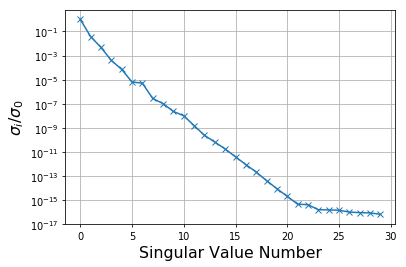
\includegraphics[scale=0.5]{singularValueSpectrum_flux.png}
	\caption{Singlar value spectrum of numerical snapshot series}
	\LFI{sv-spec}
\efg

In implementation of DMD, one often may want to use fewer modes than the $N-1$, 
	the maximum number of modes obtained without any truncation. 
Because very small singular values correspond to very little dynamics 
	information, it becomes important to understand how to choose the number of 
	dynamic modes to keep.
This can be done by specifying a relative singular value cutoff such that all 
	singular values smaller are set to zero and neglected, or by specifying the 
	number of modes desired.
If the snapshot series is denoted as $X$, and the DMD representation of $X$, 
	$X_{DMD}$, theory states that the error in the Frobenius norm should be 
	proportional to the magnitude of the largest truncated singular value, given 
	by $\lVert X - X_{DMD} \rVert_F \sim \sigma_{K+1}$ \cite{dmd2016} .
This is code verification is demonstrated in \FI{recovery}.

\bfg[h] \centering
	$
	\begin{array}{cc}
	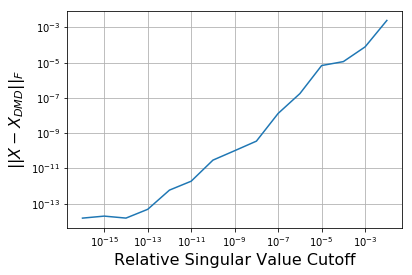
\includegraphics[scale=0.5]{cutoffStudy_flux.png} &
	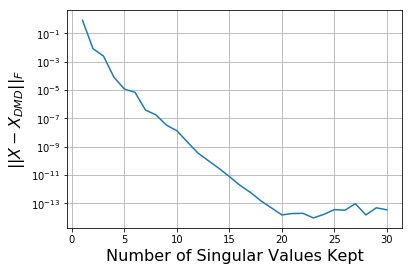
\includegraphics[scale=0.5]{rankStudy_flux.png}
	\end{array}
	$
	\caption{DMD solution recovery study}
	\LFI{recovery}
\efg

In practical applications, only the number of modes corresponding to error on 
	the order of the simulation error need be kept. 
For example, if the numerical simulation has error on the order of $10^{-4}$, 
	from the singular value spectrum above, only 5 dynamic modes are needed to 
	maintain the same level of accuracy to the analytic solution. 
For this reason, it is recommended that a singular value cutoff is used, 
	and set, to satisfy this criteria. 

To present a visual representation of DMD's ability to reproduce the solution 
	it decomposes, the DMD solution and exact solutions are plotted against each 
	other at 1/3, 1/2, and 2/3 simulation time, respectively in \FI{flx-plt}.
For this case, the numerical solution is accurate to the exact solution to 
	4 digits in an $L^2$ sense. 
This plot qualitatively shows both the accuracy of the DMD solution throughout 
	the duration of the simulation and its accuracy at times corresponding to a 
	snapshot and times in between snapshots.
%
\bfg[t] \centering
	$
	\begin{array}{cc}
	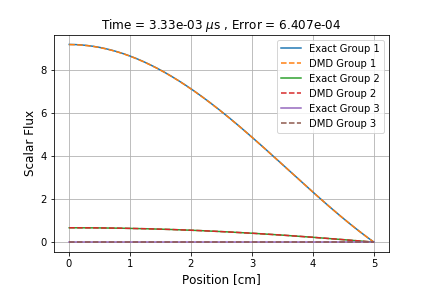
\includegraphics[scale=0.45]{groupFlux_t3ns.png} &
	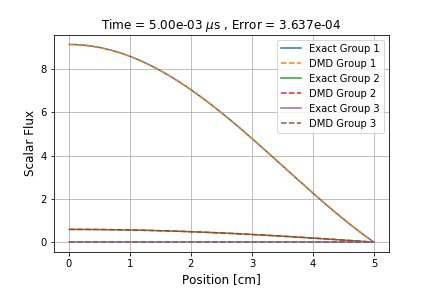
\includegraphics[scale=0.45]{groupFlux_t5ns.png} \\
	\end{array}
	$
	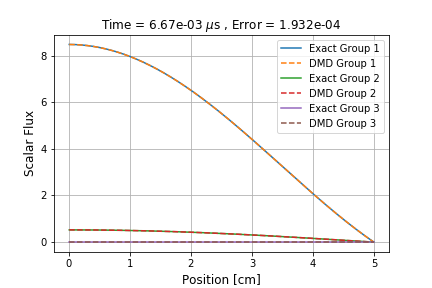
\includegraphics[scale=0.45]{groupFlux_t6ns.png}
	\caption{Scalar group flux at 1/3, 1/2, and 2/3 simulation time}
	\LFI{flx-plt}
\efg
More quantitatively, the interpolation error can be seen in \FI{interp-flux}.
In this plot, the DMD and analytic solutions are sampled on a more refined time 
	grid to obtain errors both on and in between the snapshots used to build the
	DMD solution. The DMD solution for the scalar group flux clearly does not 
	lose accuracy when interpolating between snapshots.
	%
\bfg[!htb] \centering
	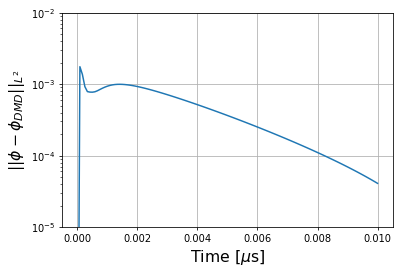
\includegraphics[scale=0.5]{flux_interp_error.png}
	\caption{Scalar group flux DMD interpolation error}
	\LFI{interp-flux}
\efg

Another property worth investigating is DMD's ability to extrapolate to times
	beyond the data collection period.
The results are presented in \FI{extrap-flux}.
%
\bfg[!htb] \centering
	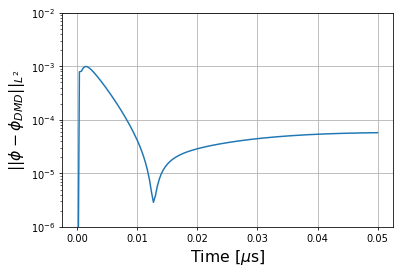
\includegraphics[scale=0.5]{flux_extrap_error.png}
	\caption{Scalar group flux DMD extrapolation error}
	\LFI{extrap-flux}
\efg
This simulation was carried out to 5 times the data collection period using the 
	same time-step size.
It is clear that DMD models this system to a similar degree of accuracy
	even very long after the sampling period.
For this case specifically, as time passes, all higher order modes become less
	relevant to the solution.
These results suggest that the DMD solution captured the dynamics of the longer
	lived modes such that as the system settles into thos modes, DMD does as well.
More information related to this is presented at a later point.

With the DMD code verified, and its capabilities thoroughly investigated, it is 
	now important to characterize its performance against the traditional 
	method used, an $\alpha$-eigenfunction expansion.
The most useful way to draw this comparison is to investigate the error of each 
	method to the exact solution as a function of number of modes.
For the $\alpha$-eigenfunction expansion, modes from the exact solution are 
	simply added in decreasing numerical order to emulate the convergence in an 
	eigenvalue solver.
To obtain the DMD-results, the SVD of the numerical data was simply truncated 
	to the appropriate rank, for the respective datapoint.
A comparison of each method is shown in \FI{comp}. 
%
\bfg[!htb] \centering
	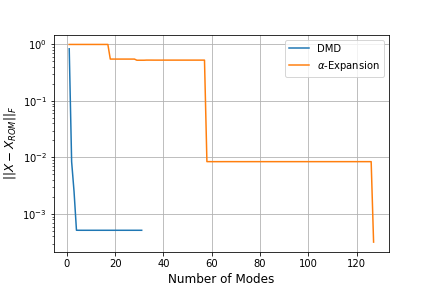
\includegraphics[scale=0.5]{method_comparison.png}
	\caption{Comparison of DMD to $\alpha$-eigenfunction expansions}
	\LFI{comp}
\efg

It is clear that DMD vastly outperforms the method of $\alpha$-eigenfunction 
	expansions.
Because eigenvalue solvers converge to eigenvalues in numerical order, many of 
	the modes converged to initially are thermally dominated and have negligible 
	contribution to the solution. 
This is what leads to the flat regions of the exact solution curve.
As is apparent, DMD rapidly converges to the error of the simulation to the 
	exact solution in fewer than 10 modes.
This is because the modes are guaranteed to be relevant to the solution over the
	simulation time, unlike $\alpha$-eigenfunctions.
If one were to increase the resolution in the numerical simulation, the minimum
	error in the DMD solution would decrease, giving it an even greater efficiency
	when compared to an $\alpha$-eigenvalue solver.

To demonstrate the ability of DMD to extract relevant structures and produce
	physical insights, the structures produced from DMD will be compared with 
	those from the $\alpha$-eigenfunction expansion.
Because no thermals exist in the system, the computed amplitudes of each 
	thermal mode is zero, however, they must still be computed before any 
	relevant modes are obtained in a standard $\alpha$-eigenvalue solver. 
The exact solution is composed of many structures which describe the physics of
	the underlying system. 
For this reason, it is expected that the DMD modes bear so resemblence to them.
To show this, the eigenvalues and eigenfunctions of the first 3 epithermal 
	modes of the $\alpha$-eigenfunction expansion and dynamic modes are compared 
	in \FI{modes}.
The epithermal modes are used becuase no thermal modes exist in the system.
The $\alpha$ modes are denoted as such, and the DMD modes denoted with $\omega$.
Each mode is normalized to its $L^2$ norm, so that an accurate comparison can 
	be made.
	
\bfg[!htb] \centering
	$
	\begin{array}{c c}
	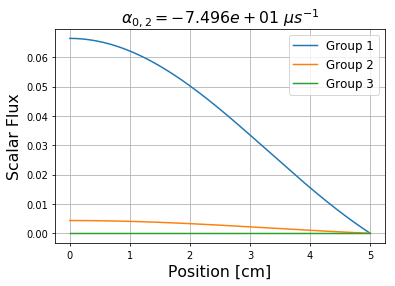
\includegraphics[scale=0.5]{alpha0-2.png} &
	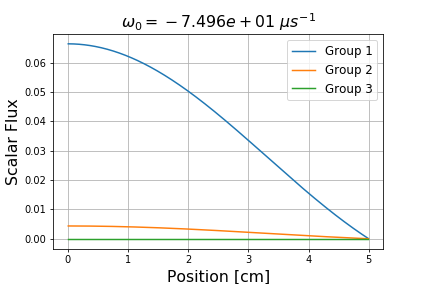
\includegraphics[scale=0.5]{dmd0.png} \\
	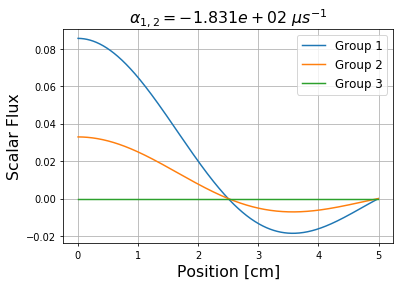
\includegraphics[scale=0.5]{alpha1-2.png} &
	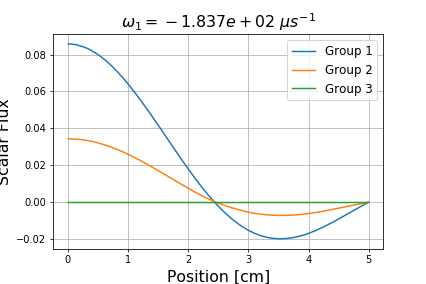
\includegraphics[scale=0.5]{dmd1} \\
	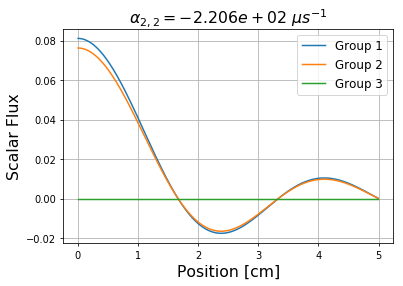
\includegraphics[scale=0.5]{alpha2-2.png} &
	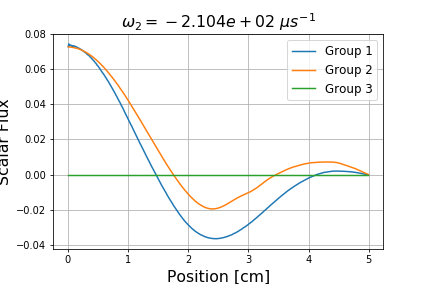
\includegraphics[scale=0.5]{dmd2.png}
	\end{array}
	$
	\caption{Comparision of $\alpha$-eigenfunctions to dynamic modes}
	\LFI{modes}
\efg

The fundamental epithermal mode and the first dynamic mode are visibly
	indistinguishable, and have identical decay constants.
The shapes of the second mode appear to be seemingly identical, and the DMD 
	decay constant is slightly different.
In the third mode, the general shape is similar but there are wide deviations 	
	in the magnitudes of each component, respectively, and again, the eigenvalue 
	further drifts away from that of the $\alpha$-eigenfunction.
Because only a finite number of dynamic modes represent the system, it is not 
	reasonable to reproduce more than a few modes accurately because the dynamic 
	modes achieve the same level of accuracy as many of the $\alpha$-eigenmode.
One could say that, in a sense, some of the dynamic modes are a combination of 	
	several	$\alpha$-eigenmodes.

These results give a clear indication of the applicability of DMD to these 
	applications.
It not only showed greater efficiency than an $\alpha$-eigenvalue computation, 
	but also preserved the physical insights which can be gained.
Further, the DMD solution produced accurate results both on and in between 
	snapshots as well as far after the sampling period.

\subsection{DMD with the Fission Rate}
For real applications, the size of solution vector may become restrictively 
large. 
For example, if one considers neutron transport, rather than diffusion, 
	increases the energy resolution,  performs a 2- or 3-D computation, or any 
	combination, the solution vector size would become exponentially larger. 
For this reason, it would be  advantageous to apply DMD on some other quantity 
	of interest, such as space-dependent reaction rates.
For this particular application, the fission rate is what primarily governs the 
	measurements of interest.
What makes this inquiry particularly interesting is the fact that no analytical
	solution exists with the same form as a DMD solution, unlike the previous
	example.
The following will present the results from the application of DMD onto the 
	fission rate computed from the scalar group flux simulation data.

As before, the singular-value spectrum should be the first check to determine 
	whether a low-rank structure exists within a given data-set. 
This is shown in \FI{sv-fis}.
%
\bfg[!htb] \centering
	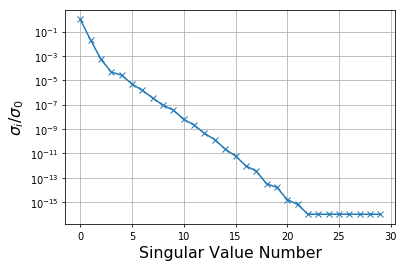
\includegraphics[scale=0.5]{singularValueSpectrum_fis.png}
	\caption{Singular value spectrum for the fission rate}
	\LFI{sv-fis}
\efg
Similarly to that for the scalar group flux, the singular value spectrum, 
	indicates that a low-rank structure exists within the space-dependent fission 
	rate snapshot series.
The error in the Frobenius norm of the DMD solution to the data which produced 
	it converges to machine precision as theory dictates.
This is shown in \FI{conv-fis}, and shows that DMD can decompose the fission
	rate as accurately as it did the scalar group flux.

\bfg[!htb] \centering
	$
	\begin{array}{c c}
	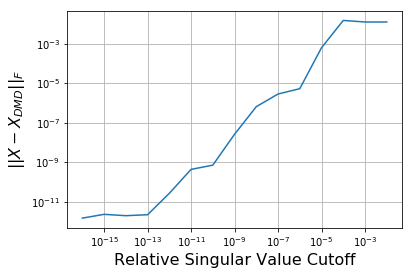
\includegraphics[scale=0.5]{cutoffStudy_fis.png}
	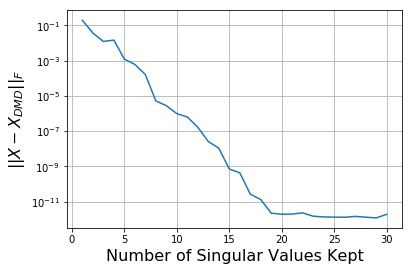
\includegraphics[scale=0.5]{rankStudy_fis.png}
	\end{array}
	$
	\caption{Fission rate DMD convergence}
	\LFI{conv-fis}
\efg

For visualization purposes, the DMD and analytic fission rates are plotted 
	against each other at 3 distinctive times, 1/3, 1/2, and 2/3 of the 
	simulation time, to depict the solution at times both on an in between times 
	corresponding to the snapshots used in DMD.
This is shown in \FI{fis-ex}.
%
\bfg[!htb] \centering
	$
	\begin{array}{c c}
	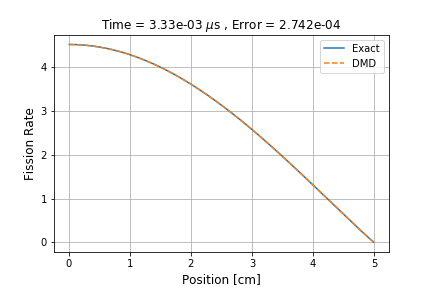
\includegraphics[scale=0.5]{fissionRate_t3ns.png}
	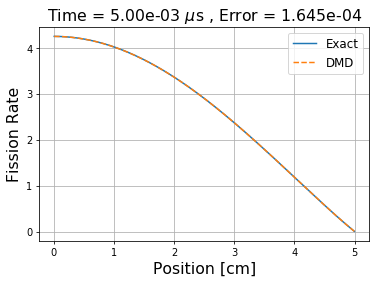
\includegraphics[scale=0.5]{fissionRate_t5ns.png}
	\end{array}
	$
	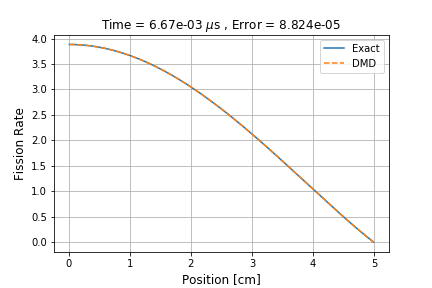
\includegraphics[scale=0.5]{fissionRate_t6ns.png}
	\caption{Fission rate at 1/3, 1/2. and 2/3 simulation time}
	\LFI{fis-ex}
\efg
The interpolative capabilities are explored in \FI{interp-fis}, and very 
similar results are obtained.

%
\bfg[!htb] \centering
	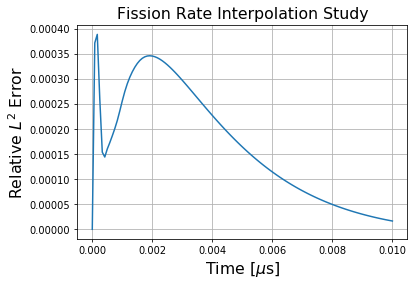
\includegraphics[scale=0.5]{fission_interp_error.png}
	\caption{Fission rate DMD interpolation error}
	\LFI{interp-fis}
\efg

Lastly, the extrapolative capabilities are explored in \FI{extrap-fis}. 
%
\bfg[t] \centering
	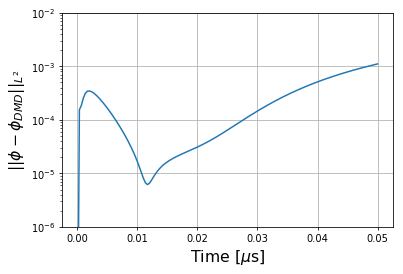
\includegraphics[scale=0.5]{fission_extrap_error.png}
	\caption{Fission rate DMD extapolation error}
	\LFI{extrap-fis}
\efg
This obviously is a very different picture than that from the scalar group flux
	extrapolation error plot.
The reason for this is believed to be because the fission rate does not have 
	a solution of the same form as the DMD solution, and therefore, as was the
	case before, the long-term behaviors cannot be sufficiently captured.
The reader should take note that the increase in error only increased by 2
	orders of magnitude after 4 times the sampling period.


\section{Conclusions and Recommendations for Future Work}
An initial study to characterize the perfomance of DMD on fast, subcritical, 
	metal systems was performed on both the scalar group flux and the fission 
	rate and to compare it to a truncated $\alpha$-eigenfunction expansion.
It was shown that not only can DMD be applied to these problems successfully,
	but that DMD shows far superior efficiency to other methods while retaining 
	the same level of physical insight.
Unlike in an $\alpha$-eigenfunction expansion, where many thermal modes with 
	zero-amplitudes must be computed before contibuting modes, dynamic modes, 
	because they are data driven, are guaranteed to be relevant to the solution.
In fact, no thermal neutrons are present in any dynamic modes.
The continuous DMD solution did not lose accuracy when interpolating between 
	snapshots, and proved to maintain accuracy for near-future state predictions.

Much work needs to be done to fully characterize DMD's applicability for these
	applications.
This work needs to be expanded to characterize non-linearities.
This is anticipated to be successful because the most notable applications of
	DMD are on turbulent fluid flow, which is nonlinear.
Further, work should be done to characterize its application to dynamic
	geometries and on coupled systems.
Lastly, the exploration of different flavors of the DMD algorithm should be 
	explored in order to find the type best suited to this application space.

\setlength{\baselineskip}{12pt}
\bibliographystyle{abbrv}
\bibliography{DMD_neutronics}

\end{document} 

